\chapter*{Adjusting Forward Rate to a Standard Temperature}

Adjusting Rates by Temperature and Activation Energy

	After "cleaning" the data for thermodynamic consistency and promixity to equilibrium, as well as limiting to the LT-WGS reaction range, the remaining data was normalized to the same temperature using the Arrhenius relationship and an approximated activation energy. 

	\begin{equation}
		rate \propto exp(\frac{-Ea}{RT}) \end{equation}
	\begin{equation}
		rate_{adj} = rate * exp(\frac{Ea/R}(\frac{1}{T} - \frac{1}{T_{adj}})) \end{equation}


	Because the LT-WGS range was define as 150C to 350C and all data points fell within this range, the adjusted temperature was decided to be 250C. Using a single activation energy to nromalize across different catallyst surfces is an assumption that introduces some amount of error. (COULD EXPLORE THIS FURTHER!). To minimize the error that this imposes on the model, a brief literature review of 16 publications was done in which 104 different activation energies for the LT-WGS reaction on various surfaces was collected [[citation]]. The results from this are given in [[fig]]. The distrbution ranged from 9 kJ/mol to 106 kJ/mol. While the results may be biased by the selected publications and the frequency with which certain surfaces were studied, the distribution should give a general indication of a good "neutral" activation energy. In \ref{fig:Ea_dist} it is shown that the most frequently cited activation energies are 40-50 kJ/mol and 60-70 kJ/mol, with both being reasonably centered in the distribution. Therefore, 70 kJ/mol was chosen as the activation energy to use to scale the forward rates. 

	\begin{figure}[]
		\centering
		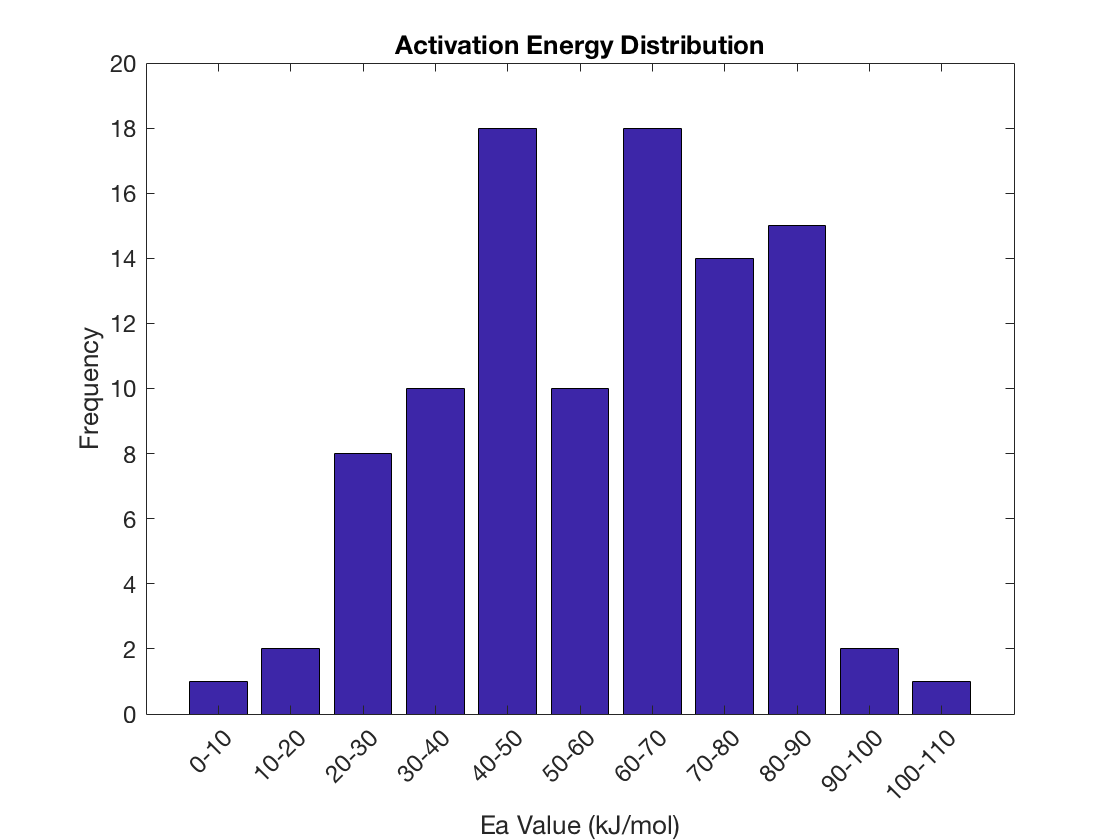
\includegraphics[width=0.5\textwidth]{TempCorrection/Ea_distribution.png}
		\caption{}
		\label{fig:Ea_dist}
	\end{figure}

	-- Why we can't remove the Temp input \& explain how this still works because it's going to bother Dumesic. 
	\begin{figure}[]
		\centering
		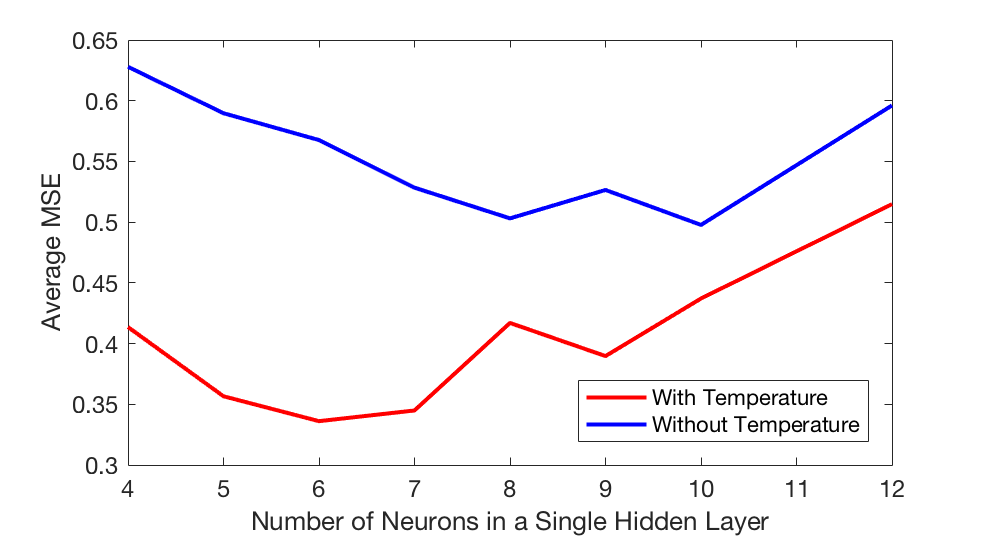
\includegraphics[width=0.6\textwidth]{TempCorrection/ChangingTempInput.png}
		\caption{}
		\label{fig:Ea_dist}
	\end{figure}